\documentclass[11pt]{article}
\usepackage[margin=1in]{geometry}
\usepackage[T1]{fontenc}
\usepackage[utf8]{inputenc}
\usepackage{graphicx}
\usepackage{enumitem}
\usepackage{hyperref}
\usepackage{parskip}

\title{GPQA Prefill Activation Projection}
\author{}
\date{2026-03-21 23:53 UTC}

\begin{document}
\maketitle

\section*{Setup}
This note summarizes the corrected activation-based visualization for the finished
2026-03-21 GPQA prompt-profile pilot. The figure is built from the saved prompt
prefill activations, not rollout text.

\begin{itemize}[leftmargin=1.5em]
\item Data source: the saved pilot bundle at
\texttt{/data/scratch/murphy/outputs/cot-loop-detection/gpqa\_s09\_prob\_pilot\_20260321/data}.
\item Prompts / rollouts: \texttt{48} prompts, \texttt{10} rollouts per prompt,
\texttt{480} rollouts total.
\item Activation object: last prefill token at the final transformer layer,
read from the saved stacked prefill shard and projected with one shared PCA plane.
\item Labels: rollout metadata from \texttt{prompt\_rollout\_archive.jsonl};
prompt-level rates from the prompt-profile JSONLs; GPQA correctness reconstructed
from the saved source rows using the recorded \texttt{sample\_id} and the same
choice-shuffle seed (\texttt{seed = 0}).
\end{itemize}

The first two PCA axes explain \texttt{15.9\%} and \texttt{9.7\%} of prompt
variance.

\section*{Main Read}
\begin{itemize}[leftmargin=1.5em]
\item Correctness is the clearest large-scale pattern in this plane. A coarse
left-vs-right slice drops from about \texttt{53.7\%} rollout correctness
(\texttt{PC1 < -4}) to \texttt{16.7\%} (\texttt{PC1 > 4}).
\item Max-length risk is visible but fragmented. The three prompts with
\texttt{p\_cap >= 0.5} sit in three distinct regions of the plane rather than in
one single failure cluster.
\item Loop risk is broader and more mixed than cap-hit risk. On this pilot every
cap hit is still a loop, but only \texttt{34 / 180 = 18.9\%} of looped rollouts
hit the cap.
\item Because repeated rollouts from one prompt share one prefill coordinate, the
plot should be read as a prompt-propensity view, not as a within-prompt branching
view.
\end{itemize}

\section*{Figures}
\begin{figure}[h]
\centering
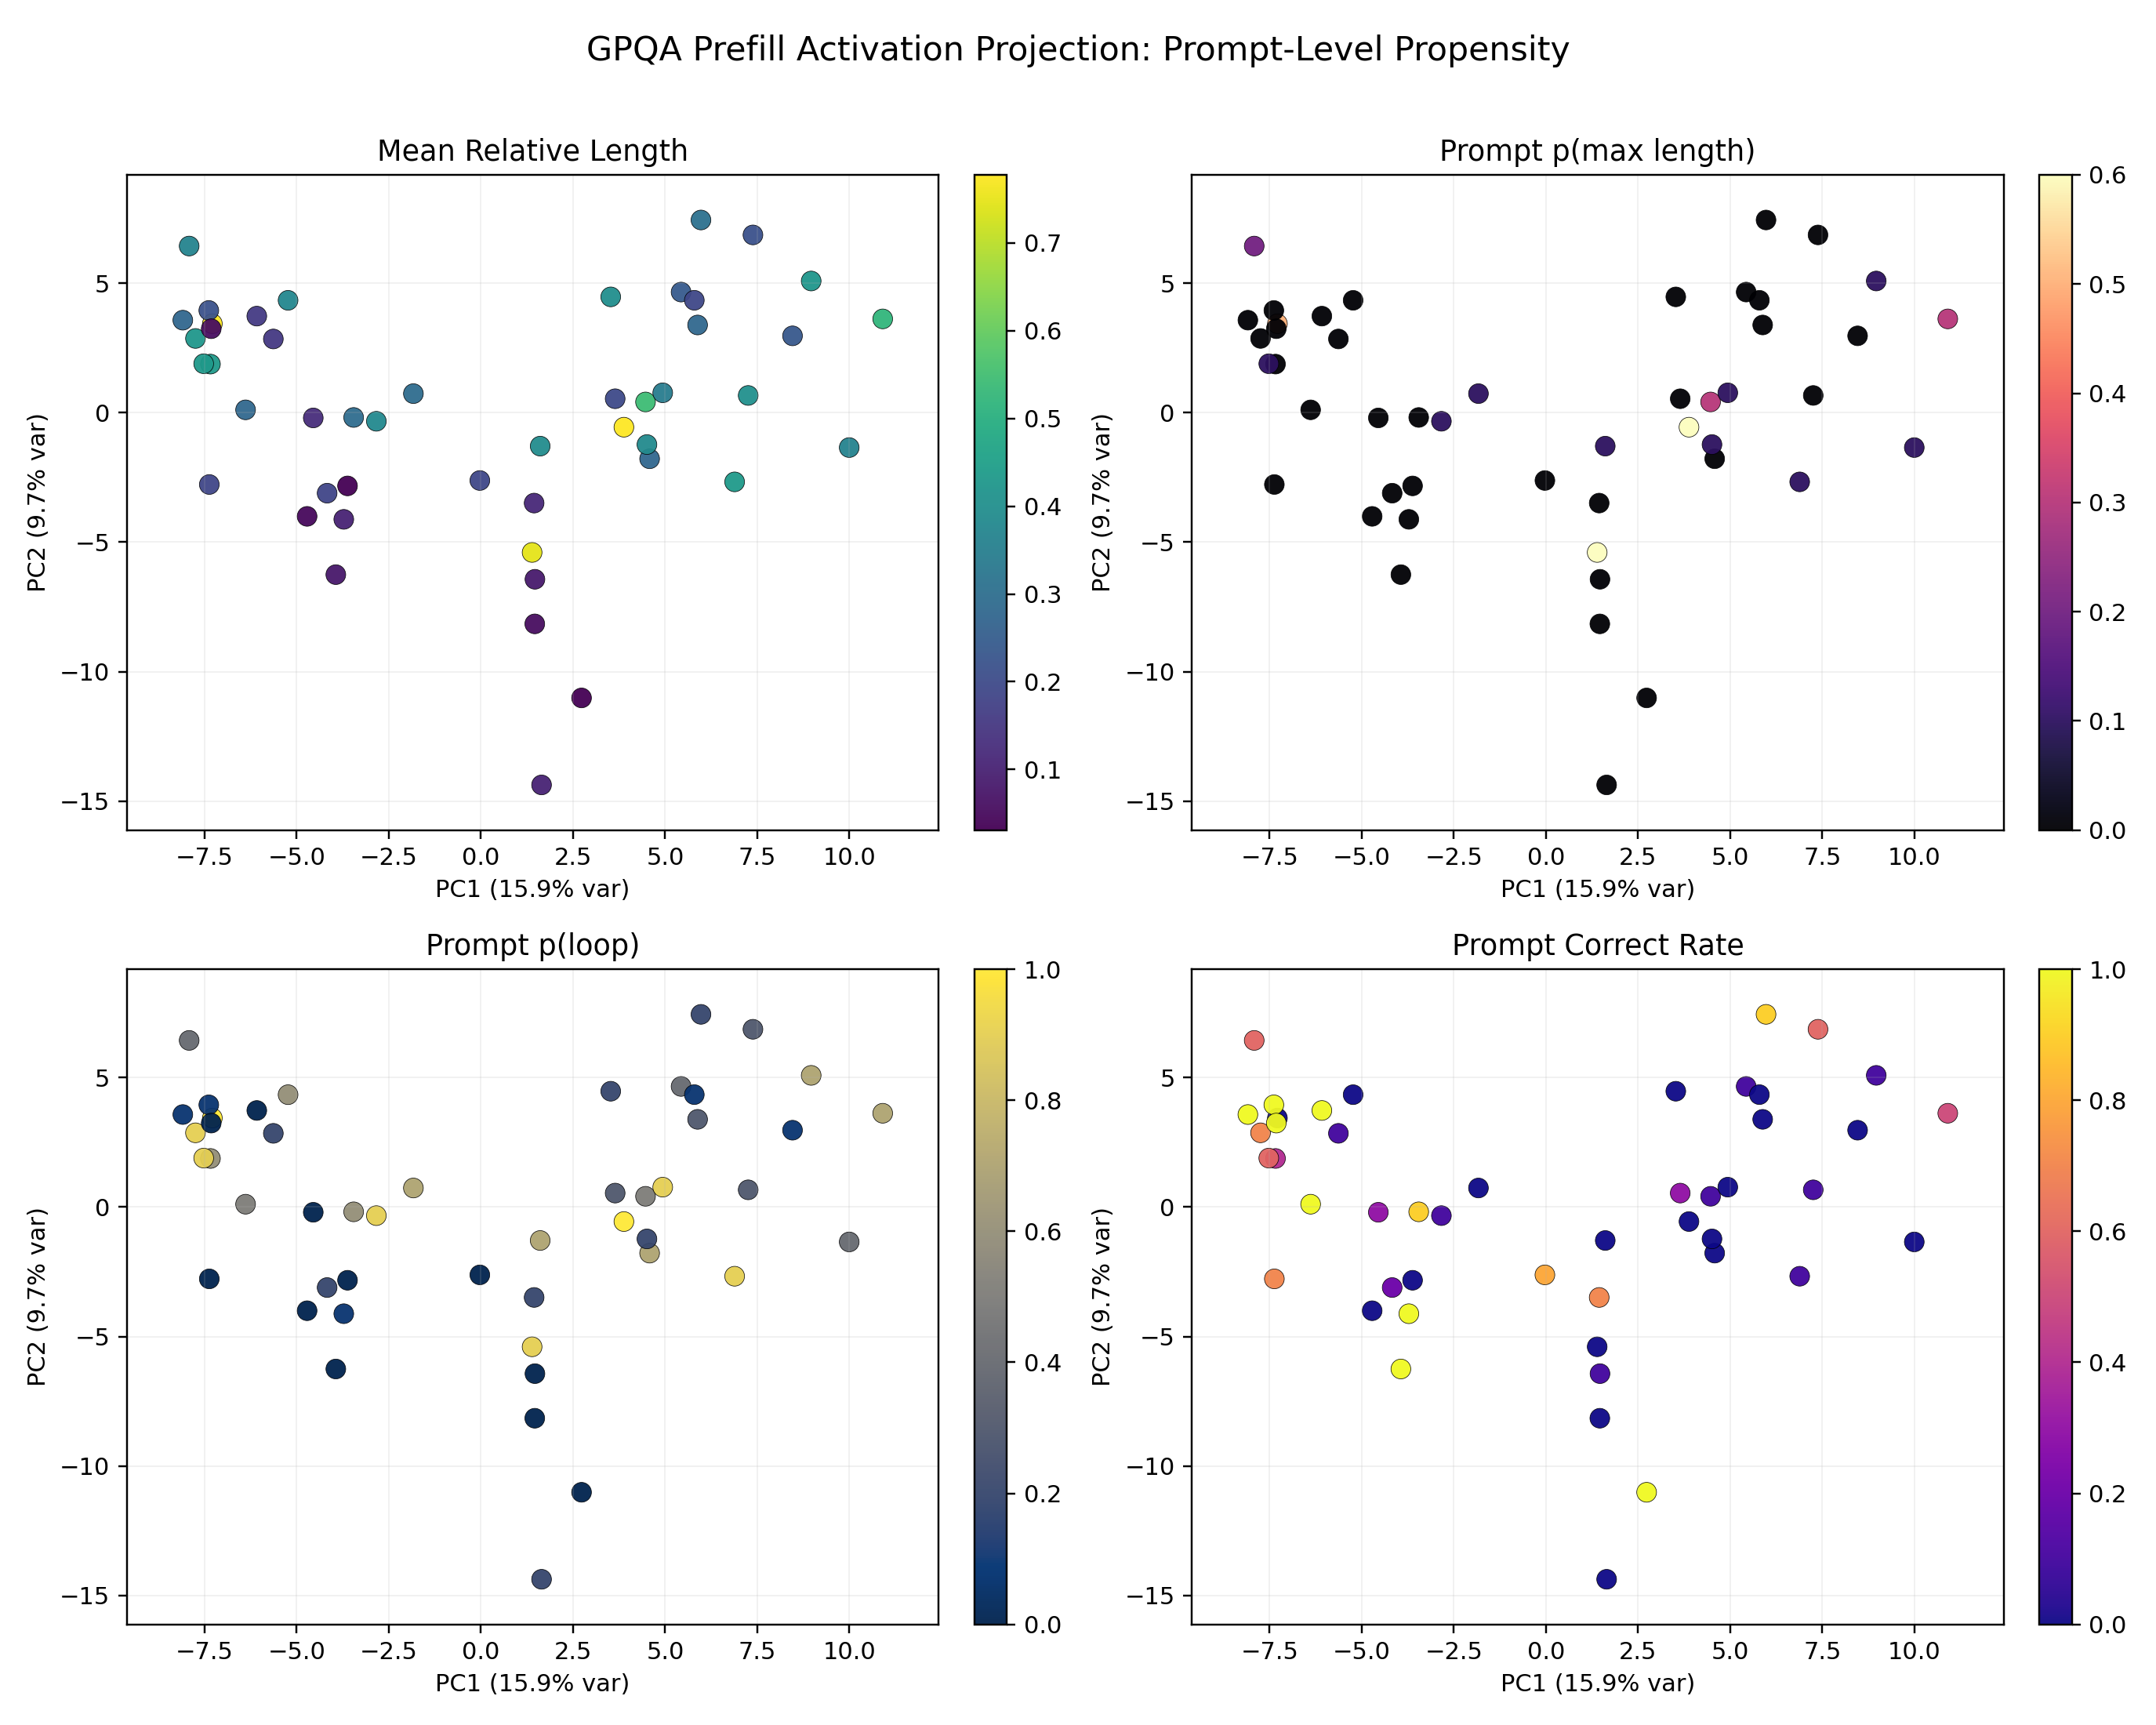
\includegraphics[width=\textwidth]{figures/prompt_projection_panels.png}
\caption{Prompt-level propensity on the shared prefill PCA plane.}
\end{figure}

\begin{figure}[h]
\centering
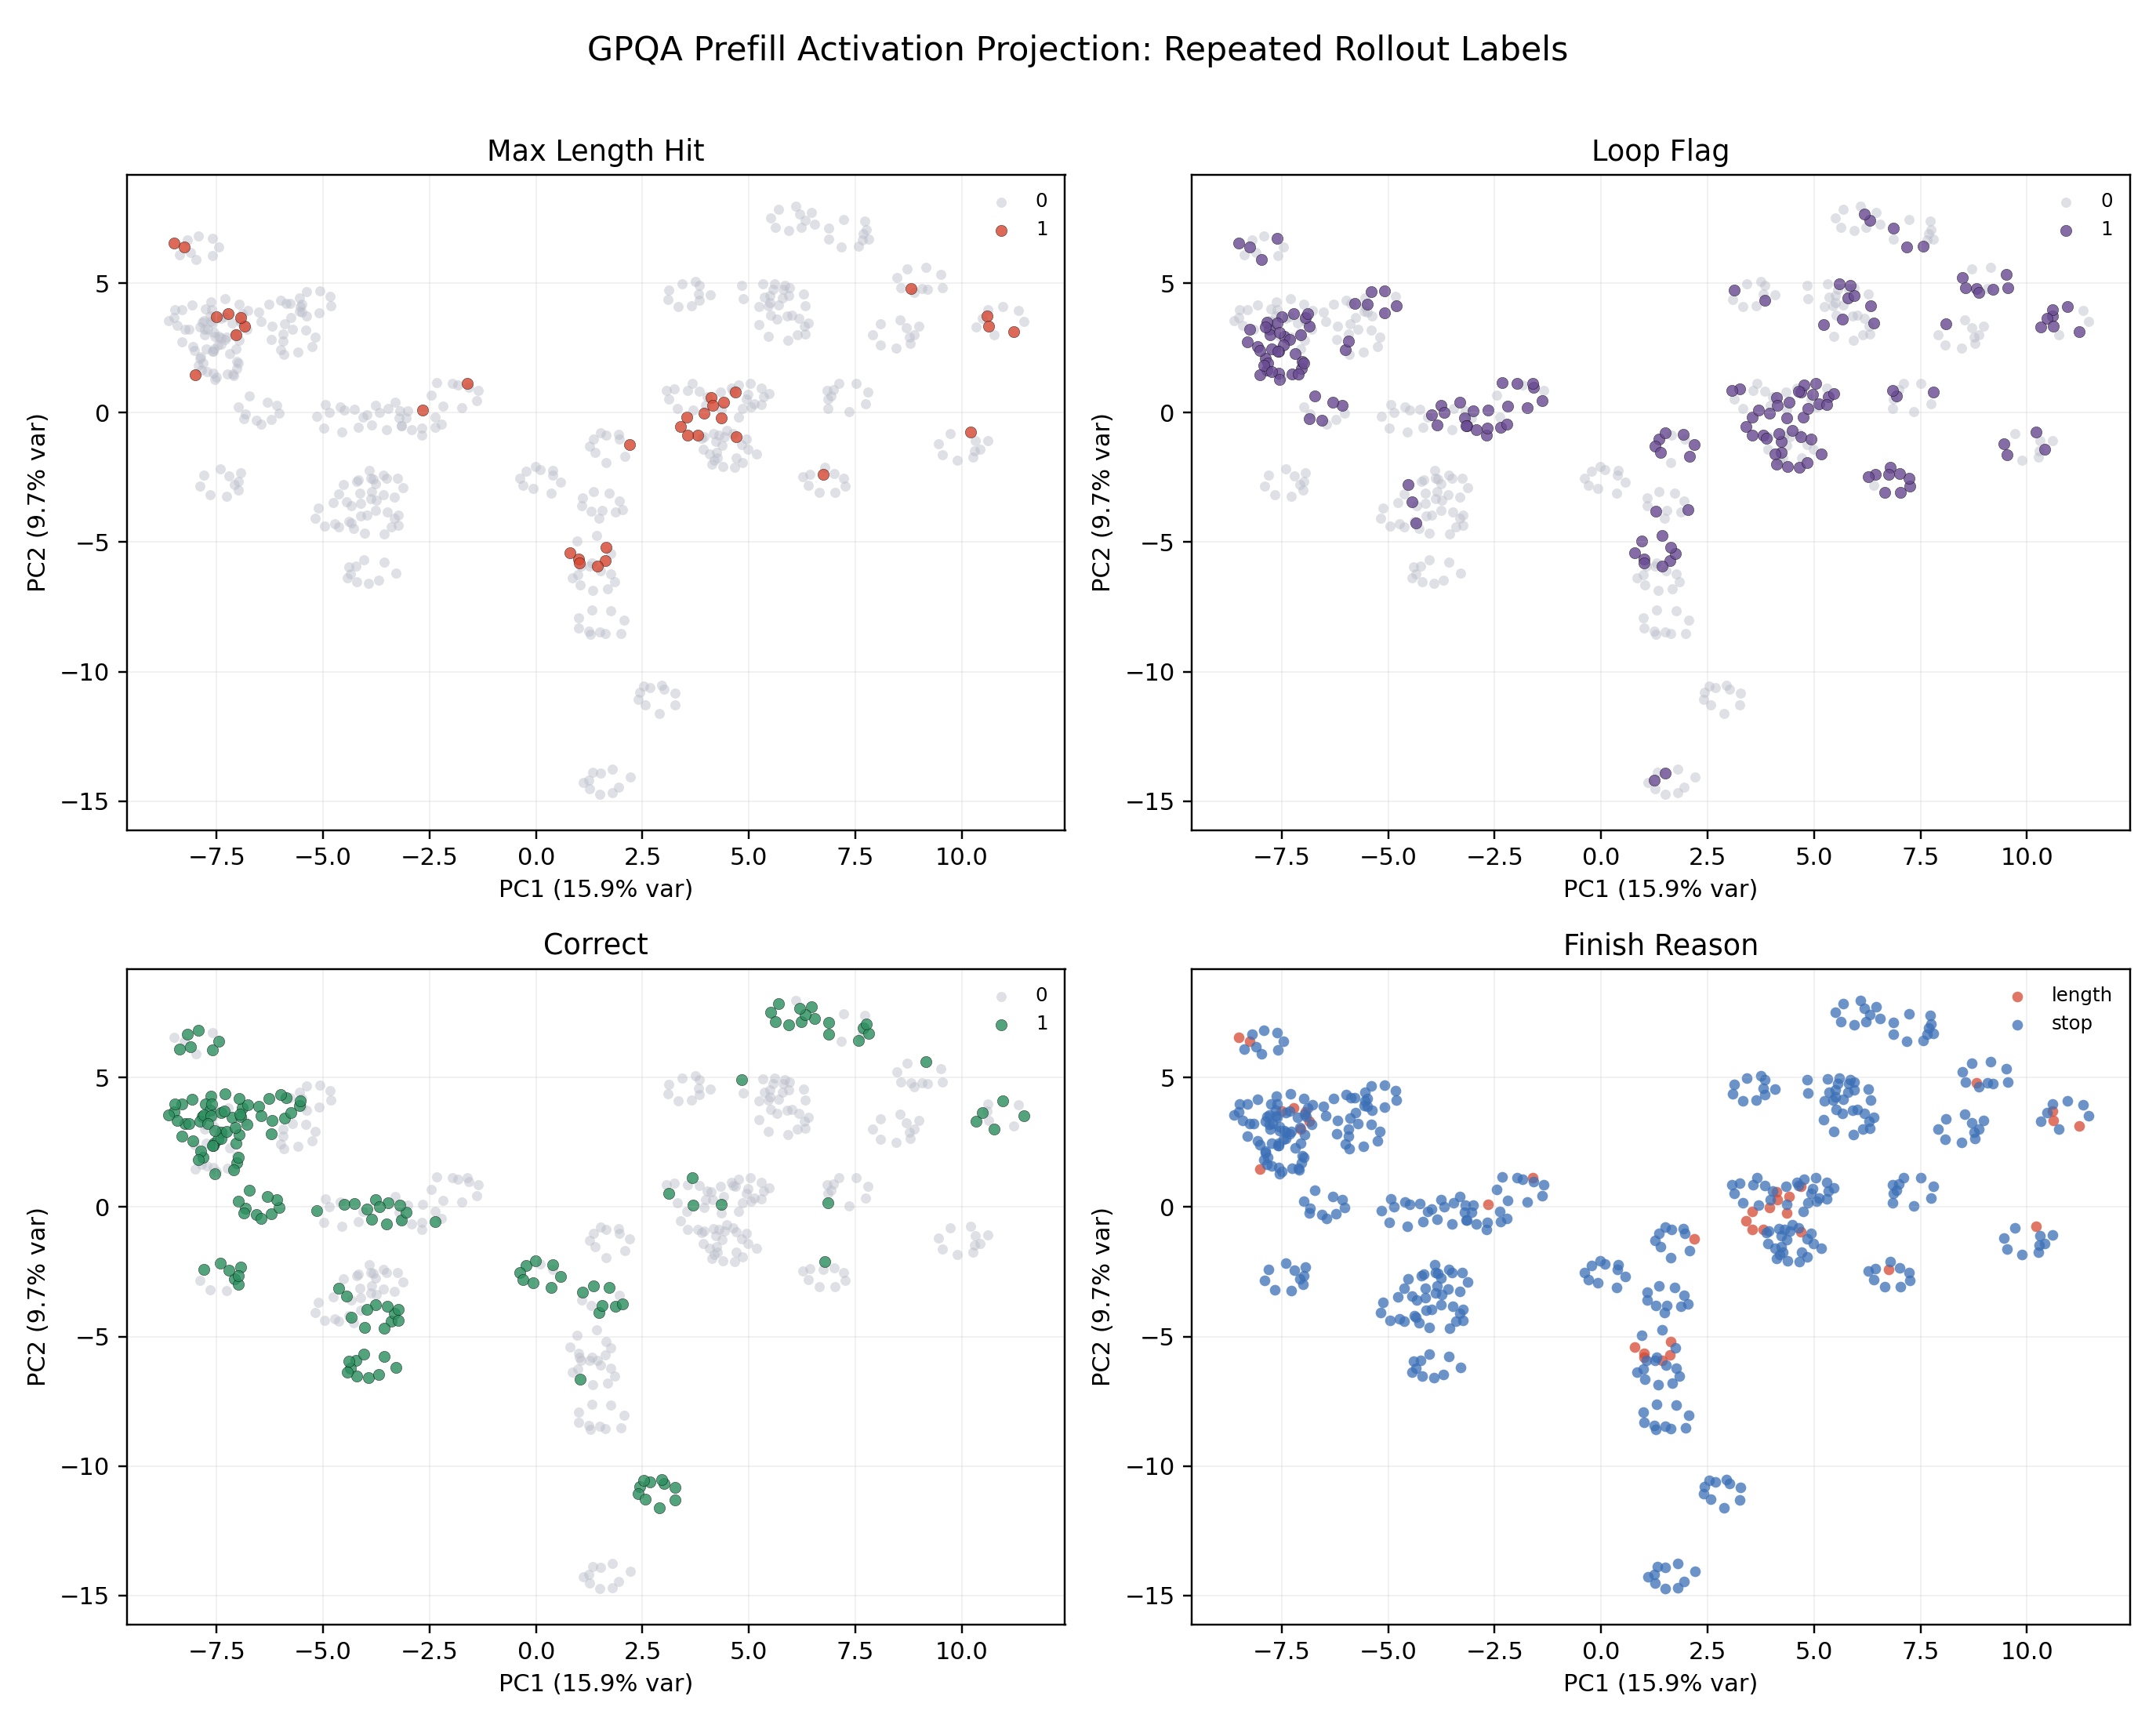
\includegraphics[width=\textwidth]{figures/rollout_projection_panels.png}
\caption{Repeated-rollout labels duplicated on the same prompt prefill coordinates
with light deterministic jitter.}
\end{figure}

\end{document}
